% CVPR 2022 Paper Template
% based on the CVPR template provided by Ming-Ming Cheng (https://github.com/MCG-NKU/CVPR_Template)
% modified and extended by Stefan Roth (stefan.roth@NOSPAMtu-darmstadt.de)

\documentclass[10pt,twocolumn,letterpaper]{article}

%%%%%%%%% PAPER TYPE  - PLEASE UPDATE FOR FINAL VERSION
\usepackage[review]{cvpr}      % To produce the REVIEW version
%\usepackage{cvpr}              % To produce the CAMERA-READY version
%\usepackage[pagenumbers]{cvpr} % To force page numbers, e.g. for an arXiv version

% Include other packages here, before hyperref.
\usepackage{graphicx}
\usepackage{amsmath}
\usepackage{amssymb}
\usepackage{booktabs}
\usepackage[UTF8]{ctex}
\usepackage{multirow}
% It is strongly recommended to use hyperref, especially for the review version.
% hyperref with option pagebackref eases the reviewers' job.
% Please disable hyperref *only* if you encounter grave issues, e.g. with the
% file validation for the camera-ready version.
%
% If you comment hyperref and then uncomment it, you should delete
% ReviewTempalte.aux before re-running LaTeX.
% (Or just hit 'q' on the first LaTeX run, let it finish, and you
%  should be clear).
\usepackage[pagebackref,breaklinks,colorlinks]{hyperref}


% Support for easy cross-referencing
\usepackage[capitalize]{cleveref}
\crefname{section}{Sec.}{Secs.}
\Crefname{section}{Section}{Sections}
\Crefname{table}{Table}{Tables}
\crefname{table}{Tab.}{Tabs.}


%%%%%%%%% PAPER ID  - PLEASE UPDATE
\def\cvprPaperID{*****} % *** Enter the CVPR Paper ID here
\def\confName{CVPR}
\def\confYear{2022}


\begin{document}

%%%%%%%%% TITLE - PLEASE UPDATE
\title{\LaTeX\ Author Guidelines for \confName~Proceedings}

\author{First Author\\
Institution1\\
Institution1 address\\
{\tt\small firstauthor@i1.org}
% For a paper whose authors are all at the same institution,
% omit the following lines up until the closing ``}''.
% Additional authors and addresses can be added with ``\and'',
% just like the second author.
% To save space, use either the email address or home page, not both
\and
Second Author\\
Institution2\\
First line of institution2 address\\
{\tt\small secondauthor@i2.org}
}
\maketitle

%%%%%%%%% ABSTRACT
\begin{abstract}
   The ABSTRACT is to be in fully justified italicized text, at the top of the left-hand column, below the author and affiliation information.
   Use the word ``Abstract'' as the title, in 12-point Times, boldface type, centered relative to the column, initially capitalized.
   The abstract is to be in 10-point, single-spaced type.
   Leave two blank lines after the Abstract, then begin the main text.
   Look at previous CVPR abstracts to get a feel for style and length.
\end{abstract}

%%%%%%%%% BODY TEXT
\section{引言}
\label{sec:intro}

引言部分

%-------------------------------------------------------------------------
\subsection{Language}

All manuscripts must be in English.

\subsection{Dual submission}

Please refer to the author guidelines on the \confName\ \confYear\ web page for a
discussion of the policy on dual submissions.

\subsection{Paper length}
Papers, excluding the references section, must be no longer than eight pages in length.
The references section will not be included in the page count, and there is no limit on the length of the references section.
For example, a paper of eight pages with two pages of references would have a total length of 10 pages.
{\bf There will be no extra page charges for \confName\ \confYear.}

Overlength papers will simply not be reviewed.
This includes papers where the margins and formatting are deemed to have been significantly altered from those laid down by this style guide.
Note that this \LaTeX\ guide already sets figure captions and references in a smaller font.
The reason such papers will not be reviewed is that there is no provision for supervised revisions of manuscripts.
The reviewing process cannot determine the suitability of the paper for presentation in eight pages if it is reviewed in eleven.

%-------------------------------------------------------------------------
\subsection{The ruler}
The \LaTeX\ style defines a printed ruler which should be present in the version submitted for review.
The ruler is provided in order that reviewers may comment on particular lines in the paper without circumlocution.
If you are preparing a document using a non-\LaTeX\ document preparation system, please arrange for an equivalent ruler to appear on the final output pages.
The presence or absence of the ruler should not change the appearance of any other content on the page.
The camera-ready copy should not contain a ruler.
(\LaTeX\ users may use options of cvpr.sty to switch between different versions.)

Reviewers:
note that the ruler measurements do not align well with lines in the paper --- this turns out to be very difficult to do well when the paper contains many figures and equations, and, when done, looks ugly.
Just use fractional references (\eg, this line is $087.5$), although in most cases one would expect that the approximate location will be adequate.


\subsection{Paper ID}
Make sure that the Paper ID from the submission system is visible in the version submitted for review (replacing the ``*****'' you see in this document).
If you are using the \LaTeX\ template, \textbf{make sure to update paper ID in the appropriate place in the tex file}.


\subsection{Mathematics}

Please number all of your sections and displayed equations as in these examples:
\begin{equation}
  E = m\cdot c^2
  \label{eq:important}
\end{equation}
and
\begin{equation}
  v = a\cdot t.
  \label{eq:also-important}
\end{equation}
It is important for readers to be able to refer to any particular equation.
Just because you did not refer to it in the text does not mean some future reader might not need to refer to it.
It is cumbersome to have to use circumlocutions like ``the equation second from the top of page 3 column 1''.
(Note that the ruler will not be present in the final copy, so is not an alternative to equation numbers).
All authors will benefit from reading Mermin's description of how to write mathematics:
\url{http://www.pamitc.org/documents/mermin.pdf}.

\subsection{Blind review}

Many authors misunderstand the concept of anonymizing for blind review.
Blind review does not mean that one must remove citations to one's own work---in fact it is often impossible to review a paper unless the previous citations are known and available.

Blind review means that you do not use the words ``my'' or ``our'' when citing previous work.
That is all.
(But see below for tech reports.)

Saying ``this builds on the work of Lucy Smith [1]'' does not say that you are Lucy Smith;
it says that you are building on her work.
If you are Smith and Jones, do not say ``as we show in [7]'', say ``as Smith and Jones show in [7]'' and at the end of the paper, include reference 7 as you would any other cited work.

An example of a bad paper just asking to be rejected:
\begin{quote}
\begin{center}
    An analysis of the frobnicatable foo filter.
\end{center}

   In this paper we present a performance analysis of our previous paper [1], and show it to be inferior to all previously known methods.
   Why the previous paper was accepted without this analysis is beyond me.

   [1] Removed for blind review
\end{quote}


An example of an acceptable paper:
\begin{quote}
\begin{center}
     An analysis of the frobnicatable foo filter.
\end{center}

   In this paper we present a performance analysis of the  paper of Smith \etal [1], and show it to be inferior to all previously known methods.
   Why the previous paper was accepted without this analysis is beyond me.

   [1] Smith, L and Jones, C. ``The frobnicatable foo filter, a fundamental contribution to human knowledge''. Nature 381(12), 1-213.
\end{quote}

If you are making a submission to another conference at the same time, which covers similar or overlapping material, you may need to refer to that submission in order to explain the differences, just as you would if you had previously published related work.
In such cases, include the anonymized parallel submission~ as supplemental material and cite it as
\begin{quote}
[1] Authors. ``The frobnicatable foo filter'', F\&G 2014 Submission ID 324, Supplied as supplemental material {\tt fg324.pdf}.
\end{quote}

Finally, you may feel you need to tell the reader that more details can be found elsewhere, and refer them to a technical report.
For conference submissions, the paper must stand on its own, and not {\em require} the reviewer to go to a tech report for further details.
Thus, you may say in the body of the paper ``further details may be found in~''.
Then submit the tech report as supplemental material.
Again, you may not assume the reviewers will read this material.

Sometimes your paper is about a problem which you tested using a tool that is widely known to be restricted to a single institution.
For example, let's say it's 1969, you have solved a key problem on the Apollo lander, and you believe that the CVPR70 audience would like to hear about your
solution.
The work is a development of your celebrated 1968 paper entitled ``Zero-g frobnication: How being the only people in the world with access to the Apollo lander source code makes us a wow at parties'', by Zeus \etal.

You can handle this paper like any other.
Do not write ``We show how to improve our previous work [Anonymous, 1968].
This time we tested the algorithm on a lunar lander [name of lander removed for blind review]''.
That would be silly, and would immediately identify the authors.
Instead write the following:
\begin{quotation}
\noindent
   We describe a system for zero-g frobnication.
   This system is new because it handles the following cases:
   A, B.  Previous systems [Zeus et al. 1968] did not  handle case B properly.
   Ours handles it by including a foo term in the bar integral.

   ...

   The proposed system was integrated with the Apollo lunar lander, and went all the way to the moon, don't you know.
   It displayed the following behaviours, which show how well we solved cases A and B: ...
\end{quotation}
As you can see, the above text follows standard scientific convention, reads better than the first version, and does not explicitly name you as the authors.
A reviewer might think it likely that the new paper was written by Zeus \etal, but cannot make any decision based on that guess.
He or she would have to be sure that no other authors could have been contracted to solve problem B.
\medskip

\noindent
FAQ\medskip\\
{\bf Q:} Are acknowledgements OK?\\
{\bf A:} No.  Leave them for the final copy.\medskip\\
{\bf Q:} How do I cite my results reported in open challenges?
{\bf A:} To conform with the double-blind review policy, you can report results of other challenge participants together with your results in your paper.
For your results, however, you should not identify yourself and should not mention your participation in the challenge.
Instead present your results referring to the method proposed in your paper and draw conclusions based on the experimental comparison to other results.\medskip\\

\begin{figure}[t]
  \centering
  \fbox{\rule{0pt}{2in} \rule{0.9\linewidth}{0pt}}
   %\includegraphics[width=0.8\linewidth]{egfigure.eps}

   \caption{Example of caption.
   It is set in Roman so that mathematics (always set in Roman: $B \sin A = A \sin B$) may be included without an ugly clash.}
   \label{fig:onecol}
\end{figure}

\subsection{Miscellaneous}

\noindent
Compare the following:\\
\begin{tabular}{ll}
 \verb'$conf_a$' &  $conf_a$ \\
 \verb'$\mathit{conf}_a$' & $\mathit{conf}_a$
\end{tabular}\\
See The \TeX book, p165.

The space after \eg, meaning ``for example'', should not be a sentence-ending space.
So \eg is correct, {\em e.g.} is not.
The provided \verb'\eg' macro takes care of this.

When citing a multi-author paper, you may save space by using ``et alia'', shortened to ``\etal'' (not ``{\em et.\ al.}'' as ``{\em et}'' is a complete word).
If you use the \verb'\etal' macro provided, then you need not worry about double periods when used at the end of a sentence as in Alpher \etal.
However, use it only when there are three or more authors.
Thus, the following is correct:
   ``Frobnication has been trendy lately.
   It was introduced by Alpher, and subsequently developed by
   Alpher and Fotheringham-Smythe, and Alpher \etal~\cite{Alpher04}.''

This is incorrect: ``... subsequently developed by Alpher \etal~\cite{Alpher03} ...'' because reference~\cite{Alpher03} has just two authors.


% Update the cvpr.cls to do the following automatically.
% For this citation style, keep multiple citations in numerical (not
% chronological) order, so prefer \cite{Alpher03,Alpher02,Authors14} to
% \cite{Alpher02,Alpher03,Authors14}.


\begin{figure*}
  \centering
  \begin{subfigure}{0.68\linewidth}
    \fbox{\rule{0pt}{2in} \rule{.9\linewidth}{0pt}}
    \caption{An example of a subfigure.}
    \label{fig:short-a}
  \end{subfigure}
  \hfill
  \begin{subfigure}{0.28\linewidth}
    \fbox{\rule{0pt}{2in} \rule{.9\linewidth}{0pt}}
    \caption{Another example of a subfigure.}
    \label{fig:short-b}
  \end{subfigure}
  \caption{Example of a short caption, which should be centered.}
  \label{fig:short}
\end{figure*}

%------------------------------------------------------------------------
\section{相关工作}
\label{sec:formatting}


%-------------------------------------------------------------------------
\subsection{Margins and page numbering}

All printed material, including text, illustrations, and charts, must be kept
within a print area $6\frac{7}{8}$ inches (17.46 cm) wide by $8\frac{7}{8}$ inches (22.54 cm)
high.
%
Page numbers should be in the footer, centered and $\frac{3}{4}$ inches from the bottom of the page.
The review version should have page numbers, yet the final version submitted as camera ready should not show any page numbers.
The \LaTeX\ template takes care of this when used properly.



%-------------------------------------------------------------------------
\subsection{Type style and fonts}

Wherever Times is specified, Times Roman may also be used.
If neither is available on your word processor, please use the font closest in
appearance to Times to which you have access.

MAIN TITLE.
Center the title $1\frac{3}{8}$ inches (3.49 cm) from the top edge of the first page.
The title should be in Times 14-point, boldface type.
Capitalize the first letter of nouns, pronouns, verbs, adjectives, and adverbs;
do not capitalize articles, coordinate conjunctions, or prepositions (unless the title begins with such a word).
Leave two blank lines after the title.

AUTHOR NAME(s) and AFFILIATION(s) are to be centered beneath the title
and printed in Times 12-point, non-boldface type.
This information is to be followed by two blank lines.

The ABSTRACT and MAIN TEXT are to be in a two-column format.

MAIN TEXT.
Type main text in 10-point Times, single-spaced.
Do NOT use double-spacing.
All paragraphs should be indented 1 pica (approx.~$\frac{1}{6}$ inch or 0.422 cm).
Make sure your text is fully justified---that is, flush left and flush right.
Please do not place any additional blank lines between paragraphs.

Figure and table captions should be 9-point Roman type as in \cref{fig:onecol,fig:short}.
Short captions should be centred.

\noindent Callouts should be 9-point Helvetica, non-boldface type.
Initially capitalize only the first word of section titles and first-, second-, and third-order headings.

FIRST-ORDER HEADINGS.
(For example, {\large \bf 1. Introduction}) should be Times 12-point boldface, initially capitalized, flush left, with one blank line before, and one blank line after.

SECOND-ORDER HEADINGS.
(For example, { \bf 1.1. Database elements}) should be Times 11-point boldface, initially capitalized, flush left, with one blank line before, and one after.
If you require a third-order heading (we discourage it), use 10-point Times, boldface, initially capitalized, flush left, preceded by one blank line, followed by a period and your text on the same line.

%-------------------------------------------------------------------------
\subsection{Footnotes}

Please use footnotes\footnote{This is what a footnote looks like.
It often distracts the reader from the main flow of the argument.} sparingly.
Indeed, try to avoid footnotes altogether and include necessary peripheral observations in the text (within parentheses, if you prefer, as in this sentence).
If you wish to use a footnote, place it at the bottom of the column on the page on which it is referenced.
Use Times 8-point type, single-spaced.


%-------------------------------------------------------------------------
\subsection{Cross-references}

For the benefit of author(s) and readers, please use the
{\small\begin{verbatim}
  \cref{...}
\end{verbatim}}  command for cross-referencing to figures, tables, equations, or sections.
This will automatically insert the appropriate label alongside the cross-reference as in this example:
\begin{quotation}
  To see how our method outperforms previous work, please see \cref{fig:onecol} and \cref{tab:example}.
  It is also possible to refer to multiple targets as once, \eg~to \cref{fig:onecol,fig:short-a}.
  You may also return to \cref{sec:formatting} or look at \cref{eq:also-important}.
\end{quotation}
If you do not wish to abbreviate the label, for example at the beginning of the sentence, you can use the
{\small\begin{verbatim}
  \Cref{...}
\end{verbatim}}
command. Here is an example:
\begin{quotation}
  \Cref{fig:onecol} is also quite important.
\end{quotation}

%-------------------------------------------------------------------------

\begin{table}
  \centering
  \begin{tabular}{@{}lc@{}}
    \toprule
    Method & Frobnability \\
    \midrule
    Theirs & Frumpy \\
    Yours & Frobbly \\
    Ours & Makes one's heart Frob\\
    \bottomrule
  \end{tabular}
  \caption{Results.   Ours is better.}
  \label{tab:example}
\end{table}

%-------------------------------------------------------------------------
\subsection{Illustrations, graphs, and photographs}

All graphics should be centered.
In \LaTeX, avoid using the \texttt{center} environment for this purpose, as this adds potentially unwanted whitespace.
Instead use
{\small\begin{verbatim}
  \centering
\end{verbatim}}
at the beginning of your figure.
Please ensure that any point you wish to make is resolvable in a printed copy of the paper.
Resize fonts in figures to match the font in the body text, and choose line widths that render effectively in print.
Readers (and reviewers), even of an electronic copy, may choose to print your paper in order to read it.
You cannot insist that they do otherwise, and therefore must not assume that they can zoom in to see tiny details on a graphic.

When placing figures in \LaTeX, it's almost always best to use \verb+\includegraphics+, and to specify the figure width as a multiple of the line width as in the example below
{\small\begin{verbatim}
   \usepackage{graphicx} ...
   \includegraphics[width=0.8\linewidth]
                   {myfile.pdf}
\end{verbatim}
}


%-------------------------------------------------------------------------
\subsection{Color}

Please refer to the author guidelines on the \confName\ \confYear\ web page for a discussion of the use of color in your document.

If you use color in your plots, please keep in mind that a significant subset of reviewers and readers may have a color vision deficiency; red-green blindness is the most frequent kind.
Hence avoid relying only on color as the discriminative feature in plots (such as red \vs green lines), but add a second discriminative feature to ease disambiguation.
%-------------------------------图片放置区
\begin{figure*}[htbp]
  \centering


  \begin{minipage}[b]{0.19\textwidth}
      \centering
      \caption*{原始白模}
  \end{minipage}
  \hfill
  \begin{minipage}[b]{0.19\textwidth}
      \centering
      
      \caption*{纹理模型}
  \end{minipage}
  \hfill
  \begin{minipage}[b]{0.19\textwidth}
      \centering
      \caption*{修改白模}
  \end{minipage}
  \hfill
  \begin{minipage}[b]{0.19\textwidth}
      \centering
      \caption*{语义模型}
  \end{minipage}\hfill
  \begin{minipage}[b]{0.19\textwidth}
      \centering
      \caption*{渲染模型}
  \end{minipage}

  \centering

  \begin{minipage}[b]{0.19\textwidth}
      \centering
      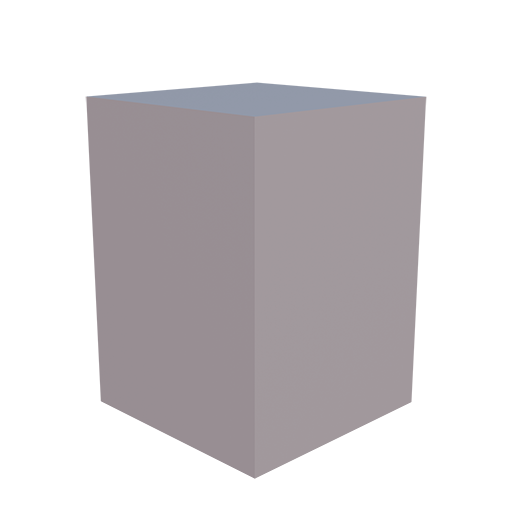
\includegraphics[width=\textwidth]{images/Bld1.png} % 替换为你的图片
  \end{minipage}
\hfill
  \begin{minipage}[b]{0.19\textwidth}
      \centering
      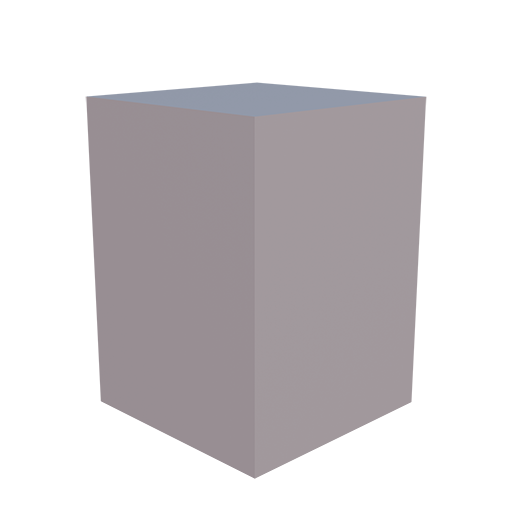
\includegraphics[width=\textwidth]{images/Bld1.png} % 替换为你的图片

  \end{minipage}
  \hfill
  \begin{minipage}[b]{0.19\textwidth}
      \centering
      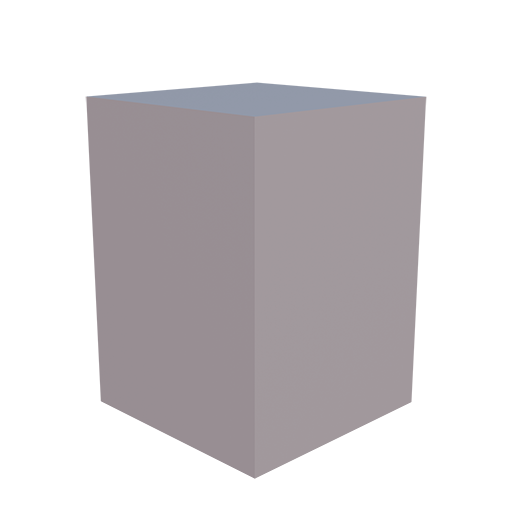
\includegraphics[width=\textwidth]{images/Bld1.png} % 替换为你的图片

  \end{minipage}
  \hfill
  \begin{minipage}[b]{0.19\textwidth}
      \centering
      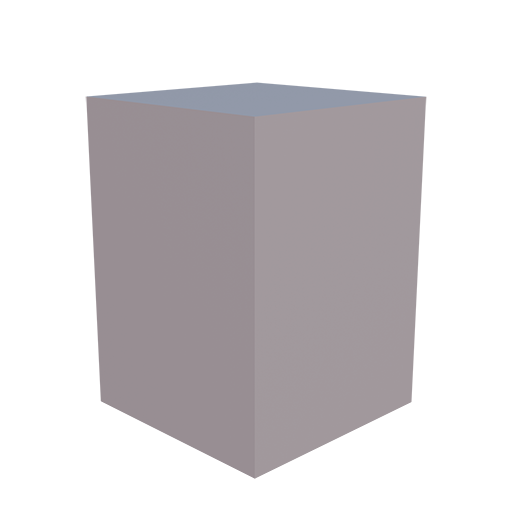
\includegraphics[width=\textwidth]{images/Bld1.png} % 替换为你的图片

  \end{minipage}
  \hfill
  \begin{minipage}[b]{0.19\textwidth}
      \centering
      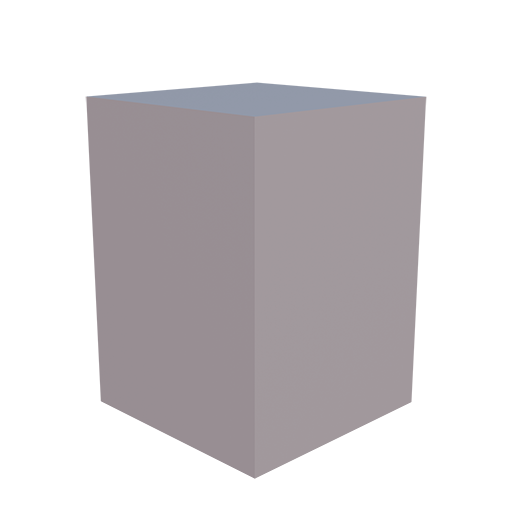
\includegraphics[width=\textwidth]{images/Bld1.png} % 替换为你的图片

  \end{minipage}
  
  \centering
  \begin{minipage}[b]{0.19\textwidth}
      \centering
      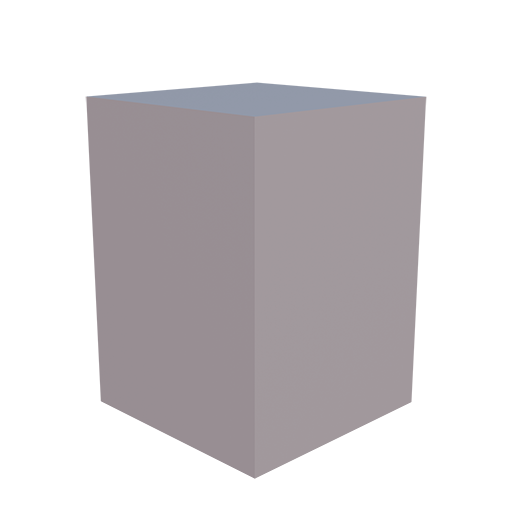
\includegraphics[width=\textwidth]{images/Bld1.png} % 替换为你的图片

  \end{minipage}
  \hfill
  \begin{minipage}[b]{0.19\textwidth}
      \centering
      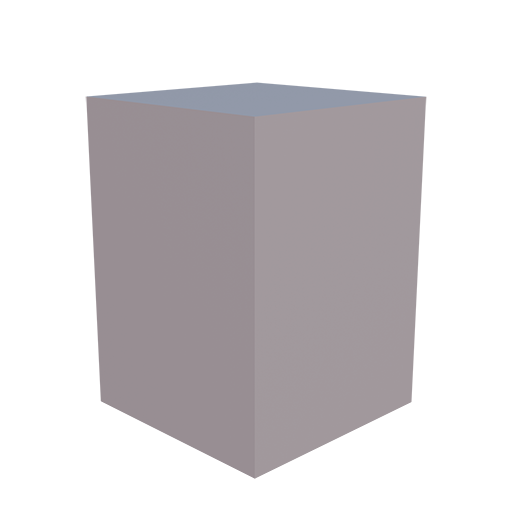
\includegraphics[width=\textwidth]{images/Bld1.png} % 替换为你的图片

  \end{minipage}
  \hfill
  \begin{minipage}[b]{0.19\textwidth}
      \centering
      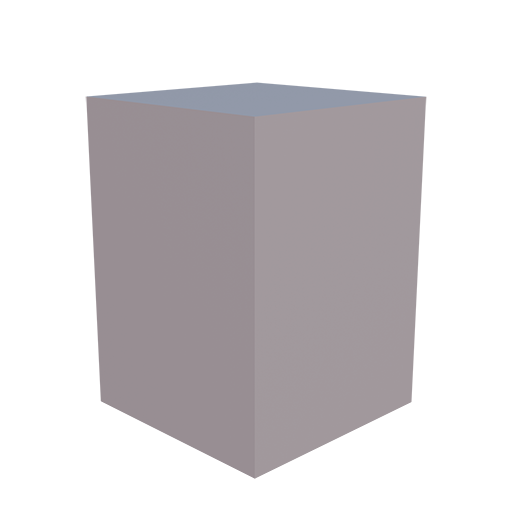
\includegraphics[width=\textwidth]{images/Bld1.png} % 替换为你的图片
  \end{minipage}
  \hfill
  \begin{minipage}[b]{0.19\textwidth}
      \centering
      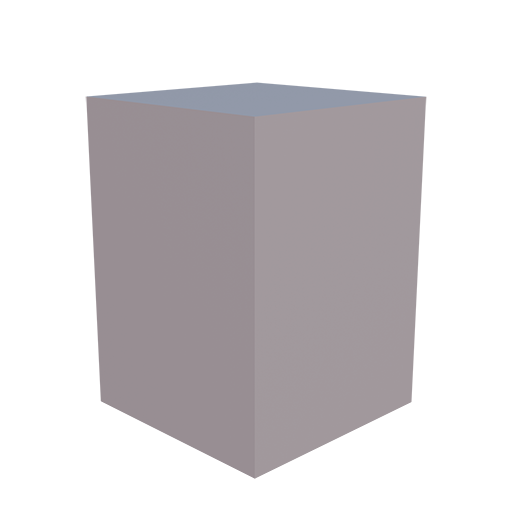
\includegraphics[width=\textwidth]{images/Bld1.png} % 替换为你的图片
  \end{minipage}
  \hfill
  \begin{minipage}[b]{0.19\textwidth}
      \centering
      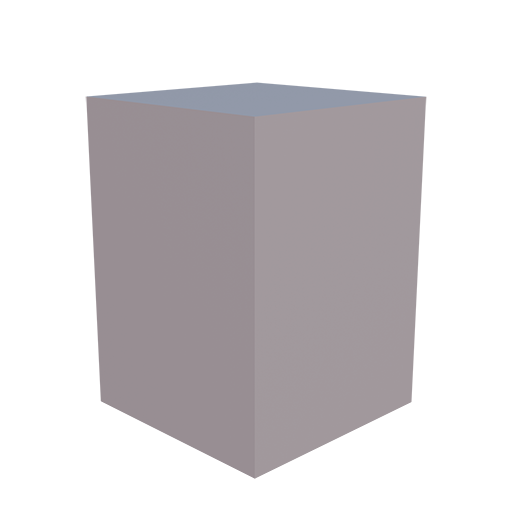
\includegraphics[width=\textwidth]{images/Bld1.png} % 替换为你的图片
  \end{minipage}
  \caption{语义建模效果示意图}
  \label{fig:row2}
\end{figure*}
%------------------------------------------------------------------------
\section{方法论}
\subsection{建筑物立面语义信息提取}

传统的语义分割方法通过像素级的分类来分配标签,能够为图像中的每个像素点提供详细的语义信息。现有的立面语义分割的研究中,通常先对立面进行语义分割,然后分析分割结果的连通语义区域,对每个连通区域计算bounding box框定语义部分~\cite{wang2024framework,mathias2016atlas,ma2022progressive}。这种方法能够提供较为精准的像素级语义标签,然而,由于分割结果会产生零碎且不连续的语义块,对于每块语义区域计算的边界框也是零碎离散的,无法保证构件级别的语义精准度,引入不必要的误差和噪声。因此我们采用YOLO架构~\cite{wang2025yolov10}目标检测方法提取立面语义,避免分割方法中的零碎问题。
\subsection{建筑物立面语义信息规则化}


\subsubsection{立面bounding box分组}
\label{sec:grouping}
在提取立面语义信息后,对得到的识别框进行立面规则化,使识别框排列分布符合一致性。首先需要对立面元素进行分组,分组过程中需要保证分组内的元素尽量一致。我们将检测框的长宽信息映射到二维平面上,形成一个二维特征空间,采用meanshift聚类方法~\cite{comaniciu2002mean}对检测框进行分类,并将meanshift邻域窗口采用矩形框的形式,尺寸设置为当前组中的平均长、宽的$\lambda$倍,这样能够确保采用meanshift方法划分每个组中立面元素具有一致的长宽比。
\begin{equation}
\bar{L}=\frac{1}{N}\sum_{i=1}^NL_i
\end{equation}
\begin{equation}
\bar{W}=\frac{1}{N}\sum_{i=1}^NW_i
\end{equation}

\begin{equation}
\text{Window Size}=\lambda\left(\frac{1}{N}\sum_{i=1}^NW_i,\frac{1}{N}\sum_{i=1}^NL_i\right)
\label{eq:groupthreshold}
\end{equation}

\begin{equation}
m(x_i)=\frac{\sum_{x_j\in W(x_i)}K(x_i-x_j)x_j}{\sum_{x_j\in W(x_i)}K(x_i-x_j)}
\label{eq:meanshift}
\end{equation}

参考~\cite{wang2024framework}立面相似元素的做法,我们将$\lambda$设为五分之一。这样就将不同尺度的窗户给区分开。此外,根据格式塔理论的邻近性和相似性原则,相似的立面构件元素在水平和垂直方向上具有一致的长或宽属性~\cite{mathias2016atlas},因而需要进一步将相似元素在水平和垂直方向上分组,以通过能量函数对齐相似元素。分组方式与之前的方法相似,若根据公式~\ref{eq:meanshift}划分出组$E:\left\{{e_{1},e_{2},e_{3},.. .,e_{n} }\right\}$,计算每个元素的质心坐标并投影到二维平面上,同样采各分组阈值$\text{Window Size}$来划分水平分组${g}_x$和垂直分组${g}_y$。
\subsubsection{分组间bounding box优化}
组间优化能量项出处~\cite{cao2017facade}基于的启发,分组间的一致性可以用分组间的最佳位移交并比IOU来衡量。
\begin
{equation}R_{ij}=\frac{R(S_i\cap T(S_j))}{R(S_i\cup T(S_j))}
\label{eq:IOUerror}
\end{equation}

其中,${R}_{ij}$表示分组${S}_i$与${S}_j$经过最佳变换${T}$后的交并比。能量函数可定义为:


\subsubsection{组内bounding box优化}
通过~\ref{sec:grouping}得到水平分组${g}_x$和垂直分组${g}_y$后,定义能量函数优化各分组的对齐性。根据水平分组${g}_x$和垂直分组${g}_y$的对齐性,边界框的水平分组中应具有相同的水平起始位置和宽度,垂直分组中应具有相同的垂直起始位置和高度。我们采用牛顿法迭代优化方法进行立面规则优化~\cite{fletcher2000practical}。
\begin{equation}
E_{x}= \sum_{g_{i} \in G }\sum_{i \in g_{i}} \left [ \left (x_{i}-\bar{x}     \right )^2+\left (w_{i}-\bar{w}    \right )^2  \right ] 
\label{eq:Ex}
\end{equation}

\begin{equation}
E_{y}= \sum_{g_{i} \in G }\sum_{i \in g_{i}} \left [ \left (y_{i}-\bar{y}    \right )^2+\left (h_{i}-\bar{h}  \right )^2  \right ]  
\label{eq:Ey}
\end{equation}

\begin{equation}
E_{total}=E_{x}+E_{y}
\label{eq:Etotal}
\end{equation}
式中,$\bar{x},\bar{w},\bar{y},\bar{h}$分别表示该水平或者垂直分组中的水平方向横坐标均值,宽度均值,左上角纵坐标均值以及高度均值。最后总的能量项${E}_{total}$为水平能量项${E}_x$和垂直能量项${E}_y$之和。

\subsection{窗户语义分割方法}

在窗户语义分割任务中,立面窗户玻璃与语义属于二分类问题,较为简单。因而采用图像分割的方法提取窗户区域的语义信息,包括窗框和玻璃。传统的图像分割方法包括区域生长、阈值法、分水岭算法、边缘检测算法,由于窗户影像颜色梯度变换较多,边缘检测算法和分水岭算法在生成生成过程会产生较多的毛躁点,无法有效区分窗框及玻璃信息,而区域生长算法难以用单一的度量指标适用不同场景。我们观察到,在大量的窗户影像中通常有着明暗区分的区域,因此采用基于otsu阈值法来进行窗户语义提取~\cite{4310076}。使用otsu阈值法并结合形态学膨胀操作能够基本提取窗户语义信息,但仍存在微小噪点。为了进一步提取干净的窗户与玻璃语义,我们采用金字塔纹理平滑~\cite{10.1145/3592120}的方法对窗户影像做预处理,再通过otsu阈值法进行二值化分割,并利用形态学开运算操作去除二值图中的微小噪声,最终得到窗户的分割掩码。随后,采用连通性分析计算每个连通区域,以bounding box作为每个连通区域的玻璃实例,并采用参数表示${\{x,y,w,h\}}$。

\subsection{建筑构件空间信息生成}
我们采用预训练的Metric3D模型~\cite{yin2023metric3d,hu2024metric3d}估计立面图像深度信息与法线信息,并结合YOLO的预测框计算为每个类计算平均深度信息,以立面深度为基准,转换窗户、门、玻璃等类别的相对深度信息。

此外,玻璃的位置信息是相对于当前窗户实例的相对位置,为了统一各个参数信息为相对于立面参数,需要进行简单转换。

对于单个建筑模型,我们构建了层次化的参数化数据结构,以表示模型的立面构件的空间位置信息,参见表~\ref{tab:facadePara}。
\begin{table}
  \centering
  \begin{tabular}{@{}lcc@{}}
    \toprule
    参数 & & 描述 \\
    \midrule
    \multirow{5}{*}{立面层} & tw & 纹理包围盒区域的宽度 \\ % 合并 window 和 door
                            & th & 纹理包围盒区域的高度 \\
                            & pw & 立面多边形的实际宽度 \\
                            & ph & 立面多边形的实际高度 \\
                            & n & 立面的法线 \\
    \multirow{2}{*}{类别层} & C& 类别 \\ % 合并 window 和 door
                            & Depth & 类别深度 \\
    \multirow{4}{*}{实例层} & x& box左上角横坐标 \\ % 合并 window 和 door
                            & y &  box左上角纵坐标 \\                                
                            & w & box宽度 \\                                
                            & h & box高度 \\                                
    \bottomrule
  \end{tabular}
  \caption{立面层次化的参数结构}
  \label{tab:facadePara}
\end{table}
\url{https://www.computer.org/about/contact}.
%------------------------------------------------------------------------
\section{实验}

%------------------------------------------------------------------------
\section{结论}
%%%%%%%%% REFERENCES
{\small
\bibliographystyle{ieee_fullname}
\bibliography{egbib}
}

\end{document}
